\documentclass{llncs}
\usepackage[T1]{fontenc}
\usepackage{graphicx}
\usepackage{enumitem}
\usepackage{amsmath}
\usepackage{listings}
\usepackage{tikz}
\usepackage{epstopdf}
\usepackage{multirow}
\usepackage{todonotes}

\title{Evaluating the Effectiveness of AEX-Notify against SGX Single-Stepping Attackers}
\author{Wicked Wench}
\institute{	University of L\"ubeck, Germany}
% TODO: For the camera-ready submission
%\author{Basil Ugbomoiko\inst{1} \quad Daniel Knaack\inst{1}}
%\institute{	University of L\"ubeck, Germany\\
%	\email{\{basil.ugbomoiko,daniel.knaack\}@student.uni-luebeck.de}}

\begin{document}

\maketitle

\begin{abstract}
  ~ \\
  \textbf{TODO}: SGX as trusted execution environment for application. Applications are executed inside enclaves. \\
  $\to$ SGX-Step as means to single-step enclaves and increase effectiveness of side-channel attacks \\
  $\to$ AEX-Notify as a mitigation for SGX-Step \\
  $\to$ Goal of the paper: Analyzing AEX-Notify and evaluating its effectiveness against SGX-Step
\end{abstract}


\section{Motivation}

Modern computing relies heavily on privileged system software to manage interactions and ensure security.
However, traditional operating system kernels are susceptible to bugs and vulnerabilities
due to their large codebase written in unsafe languages.
To address this, recent research has focused on Protected Module Architectures (PMAs),
aiming to support isolated execution of security-sensitive components
called enclaves with minimal Trusted Computing Base (TCB).
Intel’s Software Guard eXtensions (SGX) \cite{Intel16,Intel17} represent a significant advancement,
providing hardware-enforced trusted computing guarantees.
However, vulnerabilities have emerged, particularly in information leakage
through attacks exploiting various system components.
These vulnerabilities undermine the security promises of SGX.

SGX-Step presents a novel framework to address SGX vulnerabilities by enabling
precise monitoring of enclave execution at the instruction level.
Unlike previous methods, SGX-Step achieves true single-stepping for any enclave program,
significantly enhancing the resolution of existing attacks.
The framework comprises a Linux kernel driver and a runtime library,
providing the means to interrupt enclave execution at the instruction level
for detailed observation and analysis.

\paragraph{Introduction to AEX-Notify}
\begin{itemize}
  \item Overview of AEX-Notify
  \item Potential benefits of using AEX-Notify
\end{itemize}

\paragraph{Research Question and Objectives}
\begin{itemize}
  \item Formulation of the \textbf{research question}:
    Is it possible to gather control-flow information of victim programs running
    in SGX enclaves when the victim protects the execution of the enclave with
    AEX-Notify?
  \item \textbf{Project goals}:
    Our goal is to evaluate the effectiveness of AEX-Notify against SGX-step by
    constructing an example program where the SGX-Step attack works and testing
    this program once with AEX-Notify enabled and once without. We will compare
    the results to see how much information we can gain about control-flow
    information with and without AEX-Notify enabled.
\end{itemize}

\section{Background}

This section provides a comprehensive review of existing research and frameworks
relevant to the evaluation of AEX-Notify against SGX single-stepping attackers.

\subsection{Intel SGX}

Intel Software Guard Extensions (SGX) is a security feature introduced by Intel
that enables the creation of secure enclaves within applications \cite{CostanD16}.
Enclaves provide a protected execution environment for sensitive code and data,
ensuring confidentiality and integrity even if the host system is compromised.
Key components of SGX include:

\begin{itemize}
  \item \textbf{Memory Management:}
    SGX enforces memory isolation between enclaves and non-enclave code,
    preventing unauthorized access to enclave data.
  \item \textbf{Interrupt/Exception Handling:}
    SGX provides mechanisms for handling interrupts and exceptions within enclaves,
    ensuring secure execution even in the presence of external events.
  \item \textbf{TCS, SSA, TCS.CSSA:}
    SGX defines structures such as Thread Control Structure (TCS) and Saved State Area (SSA)
    to manage enclave execution and state transitions.
    \texttt{TCS.CSSA} refers to the current saved state area within the TCS.
  \item \textbf{EENTER, EEXIT:}
    SGX instructions for entering and exiting enclaves,
    facilitating the secure transition of control flow between enclave and non-enclave code.
  \item \textbf{Security Goals:}
    It's important to note that SGX's primary goal is to protect
    the confidentiality and integrity of enclave data and code,
    rather than providing defenses against side-channel attacks,
    which are the responsibility of enclave developers \cite{CostanD16}.
\end{itemize}

\subsection{SGX-Step}

SGX-Step is a framework designed to address vulnerabilities in SGX
by enabling precise monitoring of enclave execution at the instruction level \cite{ArnautovTGKMPLM16}.
Key aspects of SGX-Step include:

\begin{itemize}
    \item \textbf{Interrupting SGX Enclaves:}
      SGX-Step utilizes the APIC timer to interrupt enclave execution at specific intervals,
      allowing for detailed observation and analysis.
    \item \textbf{Challenges:}
      Previous methods for interrupting enclave execution often resulted in large time jitter,
      making it difficult to precisely control the timing of interrupts.
    \item \textbf{Improved Precision:}
      SGX-Step overcomes these challenges by configuring the APIC timer in user space,
      enabling finer control over interrupt timing and reducing time jitter \cite{ArnautovTGKMPLM16}.
\end{itemize}

\subsection{CopyCat}

CopyCat \cite{MoghimiBHPS20} is a framework that utilizes SGX-Step to extract control-flow information from SGX enclaves.
By analyzing the timing of interrupts and observing enclave behavior,
CopyCat can infer the control flow of enclave applications.

\begin{itemize}
  \item \textbf{General Idea}: Count the number of instructions on each code/data page
    and compare the page sequences of each execution with the binary to infer
    the control-flow.
  \item \textbf{Example from the paper}: If statement where else is on different page,
    the instruction sequence when the if branch is taken is $(P_0, P_0, S, P_1)$ and
    $(P_0, P_0, P_0, S, P_1)$ when else branch is taken.
  \item Attack also works for intra-page control-flow, i.e. when a branch stays
    within the same page, by counting each code page and each data page access.
\end{itemize}

\subsection{AEX-Notify}
\label{sec:aex-notify}

\begin{figure}[t]
  \centering
  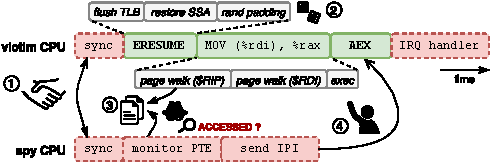
\includegraphics{images/sgx-step-pte.pdf}
  \caption{\todo[inline]{Add a proper caption here.}}
  \label{fig:sgx-step-pte}
\end{figure}

The main reason behind the effectiveness of the SGX-Step attack is the assisted
page-table walk.
Before resuming the enclave, the SGX-Step attack will clear the present bit
on the pages, which causes a page fault when executing the first instruction.
This induces additional latency in the execution of the instruction, because
the processor has to walk the page table again.
Thus, there is a large time frame where the interrupt of the timer could
arrive and land exactly on the first instruction.
The goal of AEX-Notify \cite{ConstableBCXXAK23} is to reduce the latency of the
first instruction and make it impossible to land exactly on the first
instruction.

\paragraph{Hardware Extension}
AEX-Notify introduces a new flag, called \texttt{AEXNOTIFY}, in the SSA frame.
Usually when the enclave application is resumed, the previous process context
is restored.
However, when the \texttt{AEXNOTIFY} bit is enabled, a custom exception handler
is executed.
The exception handler is responsible for handling the AEX and can resume the
application with an additional instruction, called \texttt{EDECCSSA}.
This instruction decrements \texttt{TCS.CSSA} and restores the context of the
enclave application.

\paragraph{Software Mitigation}
The goal of the mitigation is to reduce the latency of the first instruction.
In order to achieve this, it is important that the first instruction never
causes any page faults.
Otherwise, we would need to walk the page table again increasing the latency of
the instruction.
Thus, our software mitigation implements a prefetcher.
This prefetcher will always fetch necessary code and data pages of the resumed
instruction which ensures that no faults can occur.

With the software mitigation enabled, an interrupt can arrive at three possible
locations during the execution.
First, it could arrive too early and land in our prefetching code.
This would not cause any problems as resuming the enclave a second time would
call the prefetcher again and would load the same pages as before.
Next, the interrupt could arrive to late and land after the first instruction.
In this case, we would have executed more than one instruction which means
that we have successfully avoided single-stepping.
Last, it could arrive perfectly on the first instruction.
This is the exact case that we are trying to avoid.
However, since the code and data pages for this instruction have already been prefetched,
it is unlikely that an interrupt would arrive exactly on the first instruction.

\section{Work Description}

\subsection{Single-stepping Attack Implementation}

The single-stepping attack, also known as the Zigzagger attack,
aims to exploit vulnerabilities in SGX enclaves
by interrupting enclave execution at precise intervals.
This section provides a detailed overview of the Zigzagger attack methods and a step-by-step implementation guide.

\textbf{Introduction to Zigzagger Attack Methods:}
The Zigzagger attack utilizes techniques to interrupt SGX enclave execution at the instruction level,
thereby enabling the extraction of control-flow information.
It involves precise timing to resume execution either before or after specific instructions,
allowing an attacker to gather sensitive information.

\textbf{Step-by-step Implementation Guide:}
\begin{enumerate}
  \item \textbf{Identifying Target Enclaves:} The first step involves selecting target SGX enclaves susceptible to single-stepping attacks.
  \item \textbf{Setting Interrupt Intervals:} Determine the optimal timing intervals for interrupting enclave execution to capture control-flow information effectively.
  \item \textbf{Implementing Interruption Mechanism:} Develop the mechanism to interrupt enclave execution using techniques such as APIC timers.
  \item \textbf{Fine-tuning Timing:} Adjust timing parameters to ensure the interruption occurs at critical points during enclave execution.
  \item \textbf{Testing and Validation:} Validate the implementation by running test scenarios to verify the effectiveness of the single-stepping attack in extracting control-flow information.
\end{enumerate}

\subsection{Experimental Setup}

This section outlines the hardware and software specifications of the experimental environment, including configuration details necessary for conducting the evaluation.

\textbf{Hardware and Software Specifications:}
\begin{itemize}
  \item Intel Core i7 10th Gen, 16GB DDR4 RAM, and SSD storage.
  \item Ubuntu 20.04 LTS (Linux kernel version 5.10) with SGX driver support. Use SGX SDK for enclave development.
\end{itemize}

\textbf{Configuration Details:}
\begin{itemize}
  \item Configure SGX environment with appropriate BIOS settings and SGX driver installation. Utilize SGX SDK for enclave development.
  \item Set up the environment to execute the single-stepping attack. Select target enclaves and configure attack parameters for testing.
\end{itemize}

\subsection{Implementation Details for Applying AEX-Notify}

Explain how AEX-Notify is integrated into the experimental setup

\textbf{Integration with Experimental Setup:}
\begin{itemize}
  \item Integrate AEX-Notify into existing SGX environment by modifying enclave code to enable AEX-Notify functionality. Ensure compatibility with enclave execution flow and security requirements.
\end{itemize}

\textbf{Configuration and Setup Details:}
\begin{itemize}
  \item Enable AEX-Notify within the SGX enclave environment by setting appropriate flags or parameters during enclave initialization. Configure AEX-Notify to intercept and handle exceptions caused by single-stepping attacks.
\end{itemize}

We enable AEX-Notify by adding an additional field in the enclave configuration.
The exception handler is preconfigured to use the trusted runtime system of the SDK.
This is the same handler as described in Section~\ref{sec:aex-notify}.

\section{Results}

\begin{itemize}
  \item After enabling AEX-Notify, we can no longer single-step (This is the most basic requirement, so not really special)
  \item The interrupt lands in the exception handler most of the time
  \item For pages without any return, the interrupt arrives during the C3 cache lookup.
  \item \textbf{TODO}: Where does the exception handler rollback when interrupting the small assembly stub?
  \item \textbf{TODO}: Can we differentiate between zero-step and multi-step by simulating a cache attack?
\end{itemize}

\section{Conclusion and Future Work}
\begin{itemize}
    \item Summary of key findings
    \item Potential enhancements to AEX-Notify
    \item Future research directions
\end{itemize}

\bibliographystyle{alpha}
%\bibliographystyle{splncs03}
\bibliography{references}
\end{document}
